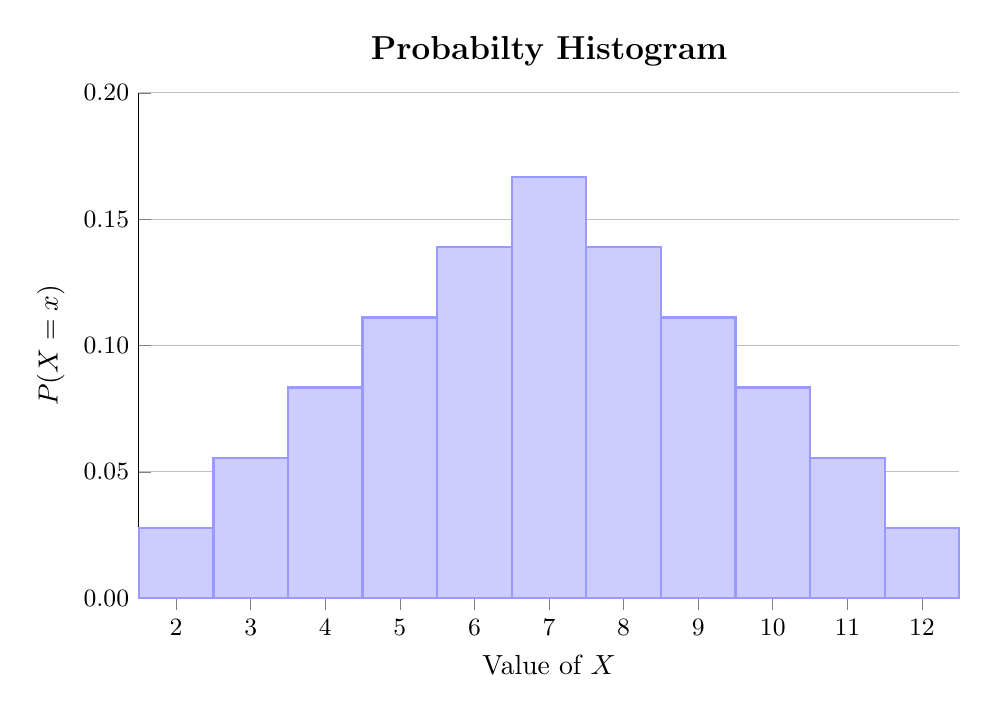
\begin{tikzpicture}
  \begin{axis}[
      axis lines*=left,
      no markers,
      xmin=1.5, xmax=12.5, ymin=0, ymax=0.2,
      xtick={2,...,12},
      ytick={0,0.05,0.1,0.15,0.2},
      xlabel={Value of $X$},
      ylabel={$P(X=x)$},
      title={\large\bf Probabilty Histogram},
      ticklabel style={font=\small},
      y tick label style={
        /pgf/number format/.cd,
        fixed,
        fixed zerofill,
        precision=2,
        /tikz/.cd
      },
      enlargelimits=false,
      clip=false,
      grid = none,
      ymajorgrids=true,
      ybar=0pt,
      bar width=1,
      width=12cm,
      height=8cm
    ]
    \addplot+[thick,fill=blue!20,draw=blue!40]  coordinates { 
      (2,{1/36})
      (3,{2/36})
      (4,{3/36})
      (5,{4/36})
      (6,{5/36})
      (7,{6/36})
      (8,{5/36})
      (9,{4/36})
      (10,{3/36})
      (11,{2/36})
      (12,{1/36})
    };
  \end{axis}
\end{tikzpicture}
